\newpage
\begin{appendices}


% \section{Proofs}

% \subsection{---} \label{Proofs:}



%\newpage
\section{Homeworks}
\subsection{For Section 1}

\begin{question}\label{question:graph-equivelance}
    \textbf{Show equivalence between the factorization and conditional independence over G in the Scores of units example:} \\
    First we will create G using the following factorization:
    \begin{equation}
        p(\text{Maths}, \text{SM}1, \text{Python}, \text{ML}) \propto g_{1}(\text{Maths}, \text{SM}1) \cdot g_{2}(\text{Python}, \text{ML}, \text{SM}1)
    \end{equation}
    The graph corresponding to this factorization is:
    \begin{figure}[h]
    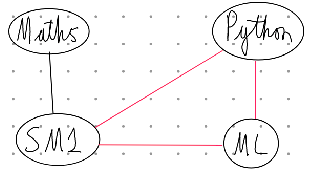
\includegraphics[width=\textwidth/2]{images/factor_graph.png}
    \centering
    \end{figure}
    Where in black is the edges corresponding to the clique given by the first factor and in red the edges corresponding to the clique given by the second factor. The conditional independencies encoded by this graph are:
    \begin{enumerate}
        \item Maths $\bot$ Python $|$ SM1
        \item Maths $\bot$ Python $|$ SM1, ML 
        \item Maths $\bot$ ML $|$ SM1
        \item Maths $\bot$ ML $|$ SM1 , Python
        \item Maths $\bot$ ML, Python $|$ SM1
    \end{enumerate}
    Which are all the conditional independencies of $p(\text{Maths}, \text{SM}1, \text{Python}, \text{ML})$. 

    Now we will create G using all the conditional independencies, which are:
    \begin{enumerate}
        \item Maths $\bot$ Python $|$ SM1
        \item Maths $\bot$ Python $|$ SM1, ML 
        \item Maths $\bot$ ML $|$ SM1
        \item Maths $\bot$ ML $|$ SM1 , Python
        \item Maths $\bot$ ML, Python $|$ SM1
    \end{enumerate}
    The graph we get is the same as before, and reading the graph its clear that it encodes the factorization of $p(\text{Maths}, \text{SM}1, \text{Python}, \text{ML})$. Hence, shown.
\end{question}

\subsection{For Section 2}
\begin{question}
    \textbf{Suppose graph G encodes all conditional independencies in your Gaussian distribution $p(\x)$. Let's say G contains 3 edges and 5 nodes. How many non-zero elements are there in inverse covariance matrix of p?:} \\
    There are 25 entries in $\bm{\Theta}$ and in the adjacency matrix of G (also with 25 entries) there are 6 non-zero (ie. equal to 1) entries hence only 6 entries in $\bm{\Theta}$ that are non-zero (from \cref{equation:adjacency-Theta}). 
\end{question}

\begin{question}\label{question:logistic-regression}
    \textbf{In \cref{subsubsection:Logistic-Regression} we constructed a logistic regression from our simple Markov network model where $\hat{\bm{\beta}}, \hat{\beta_{0}} = \argmax_{\bm{\beta}, \beta_{0}} \sum_{i=1}^{n} \log(p(y_{i}|\xui;\bm{\beta},\beta_{0}))$ show that this is the same logistic regression we talked about in portfolio 3:} \\
    Note that we can write:
    \begin{equation}
        p(y=-1| \x) = 1 / (1+ \frac{p(\x|y=+1)p(y=+1)}{p(\x|y=-1) p(y=-1)})
    \end{equation}
    And for $p(y=-1|\x)$ the same is true but with the inverse of the ratio of the densities. We can rewrite this more generally as:
    \begin{equation}
        p(y | \x; \bm{\beta}, \beta_{0}) = \sigma(f(\x;\bm{\beta}, \beta_{0}) \cdot y)
    \end{equation}
    where $f(\x;\bm{\beta}, \beta_{0}) = log( [p(\x|y=+1)p(y=+1)] / [p(\x|y=-1) p(y=-1)] )$. Hence we can rewrite our MLE as the logistic regression:
    \begin{equation}
        \hat{\bm{\beta}}, \hat{\beta_{0}} = \argmax_{\bm{\beta}, \beta_{0}} \sum_{i=1}^{n} \log (\sigma(f(\xui;\bm{\beta}, \beta_{0}) \cdot y_{i}))
    \end{equation}
    Which is the same logistic regression we had in portfolio 3.
\end{question}


\subsection{For Section 3}
\begin{question}
    \textbf{Given the simple Bayesian Network model described in \cref{section:Bayesian-Network}, however, now with one additional node $X'$ which has one inbound directed edge from $X^{(1)}$. Given this Bayesian Network for a classification task, should you include feature $X'$ for classification? and why?} \\
    To be able to solve the classification problem we would like to find $p(Y|X)$ which for this Bayesian Network is equal to:
    \begin{equation}
        P(Y|X) = \frac{\prod_{i} P(X^{(i)} | Y) P(Y)P(X' | X^{(1)}) }{P(X)}
    \end{equation}
    Hence, we should include feature $X'$ for classification as our factorization and therefore prediction depends on it. 
\end{question}


\end{appendices}